\subsection{AK jet mass distributions}

The results on the jet mass distributions in this section and below are reported in several different $p_T$ regions for the leading jet: $(1) 125 < p_T < 200$ GeV, $(1) 200 < p_T < 300$ GeV, $(1) 300 < p_T < 400$ GeV, and $(1) p_T >400$ GeV.
We start by showing in fig.~\ref{figs:allAlgos1}-\ref{figs:allAlgos3} the reconstructed ``raw'' ungroomed and grommed mass distributions on data for AK5, AK7 and AK8 jets.

\begin{figure}[!htb]
\centering
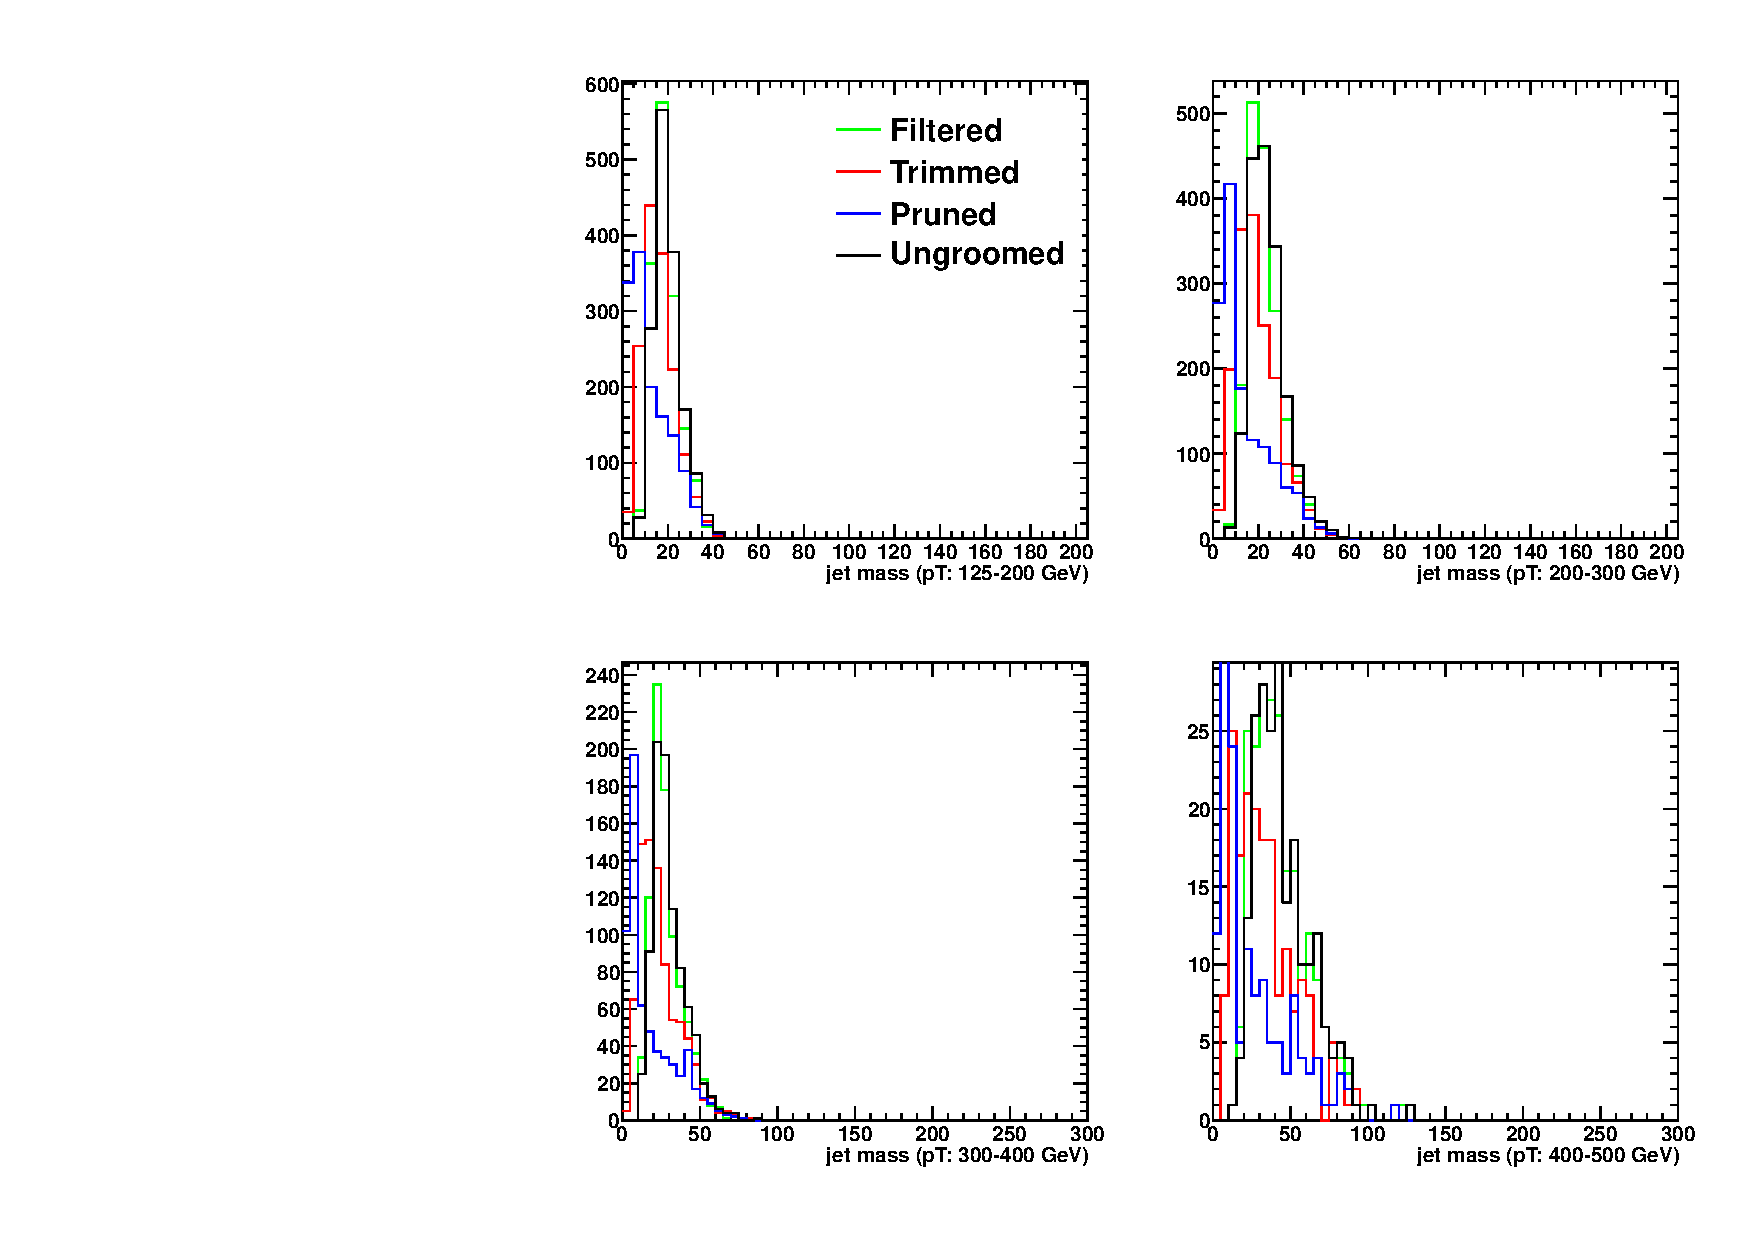
\includegraphics[width=1.0\textwidth]{figs/allAlgos_2x2PtBins_ak5.pdf}
\caption{Raw jet mass distribution on data for the leading AK5 (ungroomed or groomed) jet in different jet momentum regions.}
\label{figs:allAlgos1}
\end{figure}

\begin{figure}[!htb]
\centering
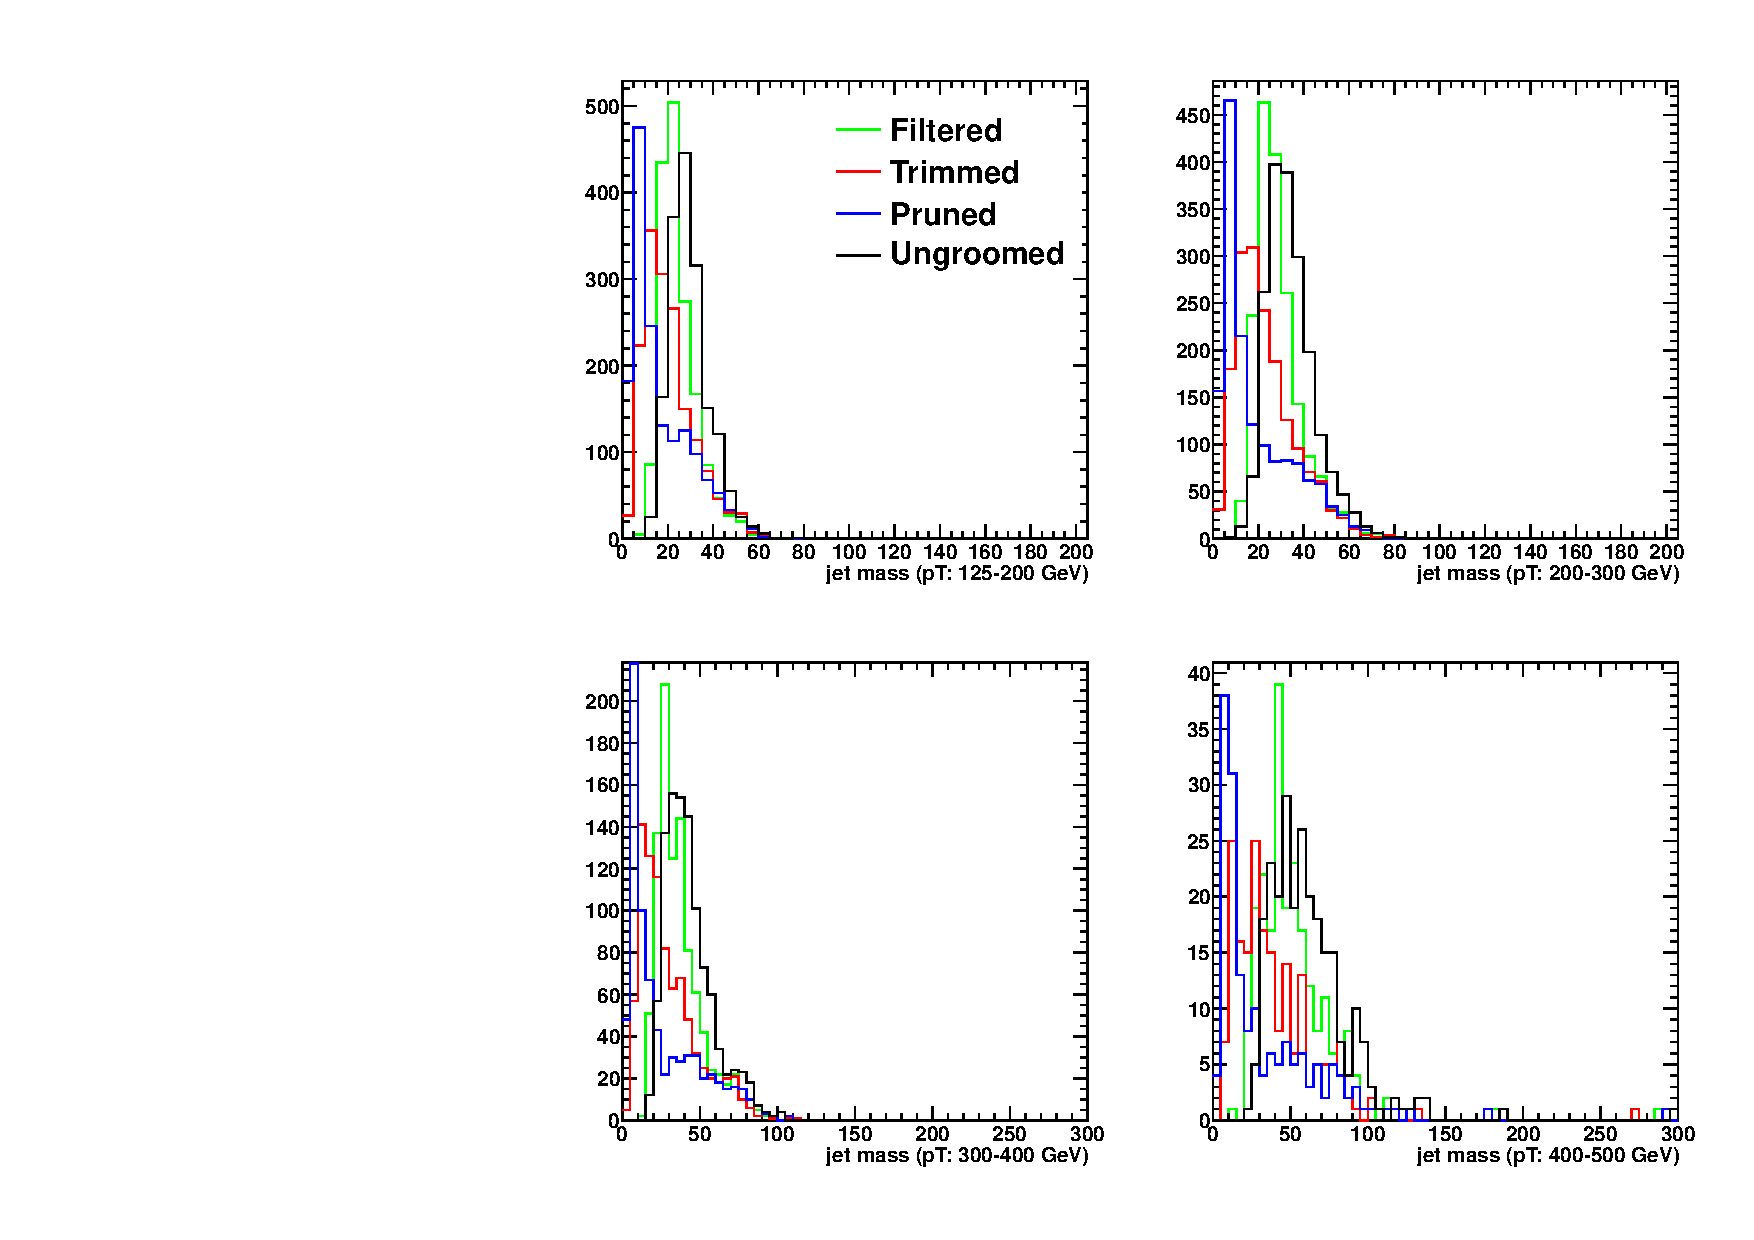
\includegraphics[width=1.0\textwidth]{figs/allAlgos_2x2PtBins_ak7.pdf}
\caption{Raw jet mass distribution on data for the leading AK7 (ungroomed or groomed) jet in different jet momentum regions.}
\label{figs:allAlgos2}
\end{figure}

\begin{figure}[!htb]
\centering
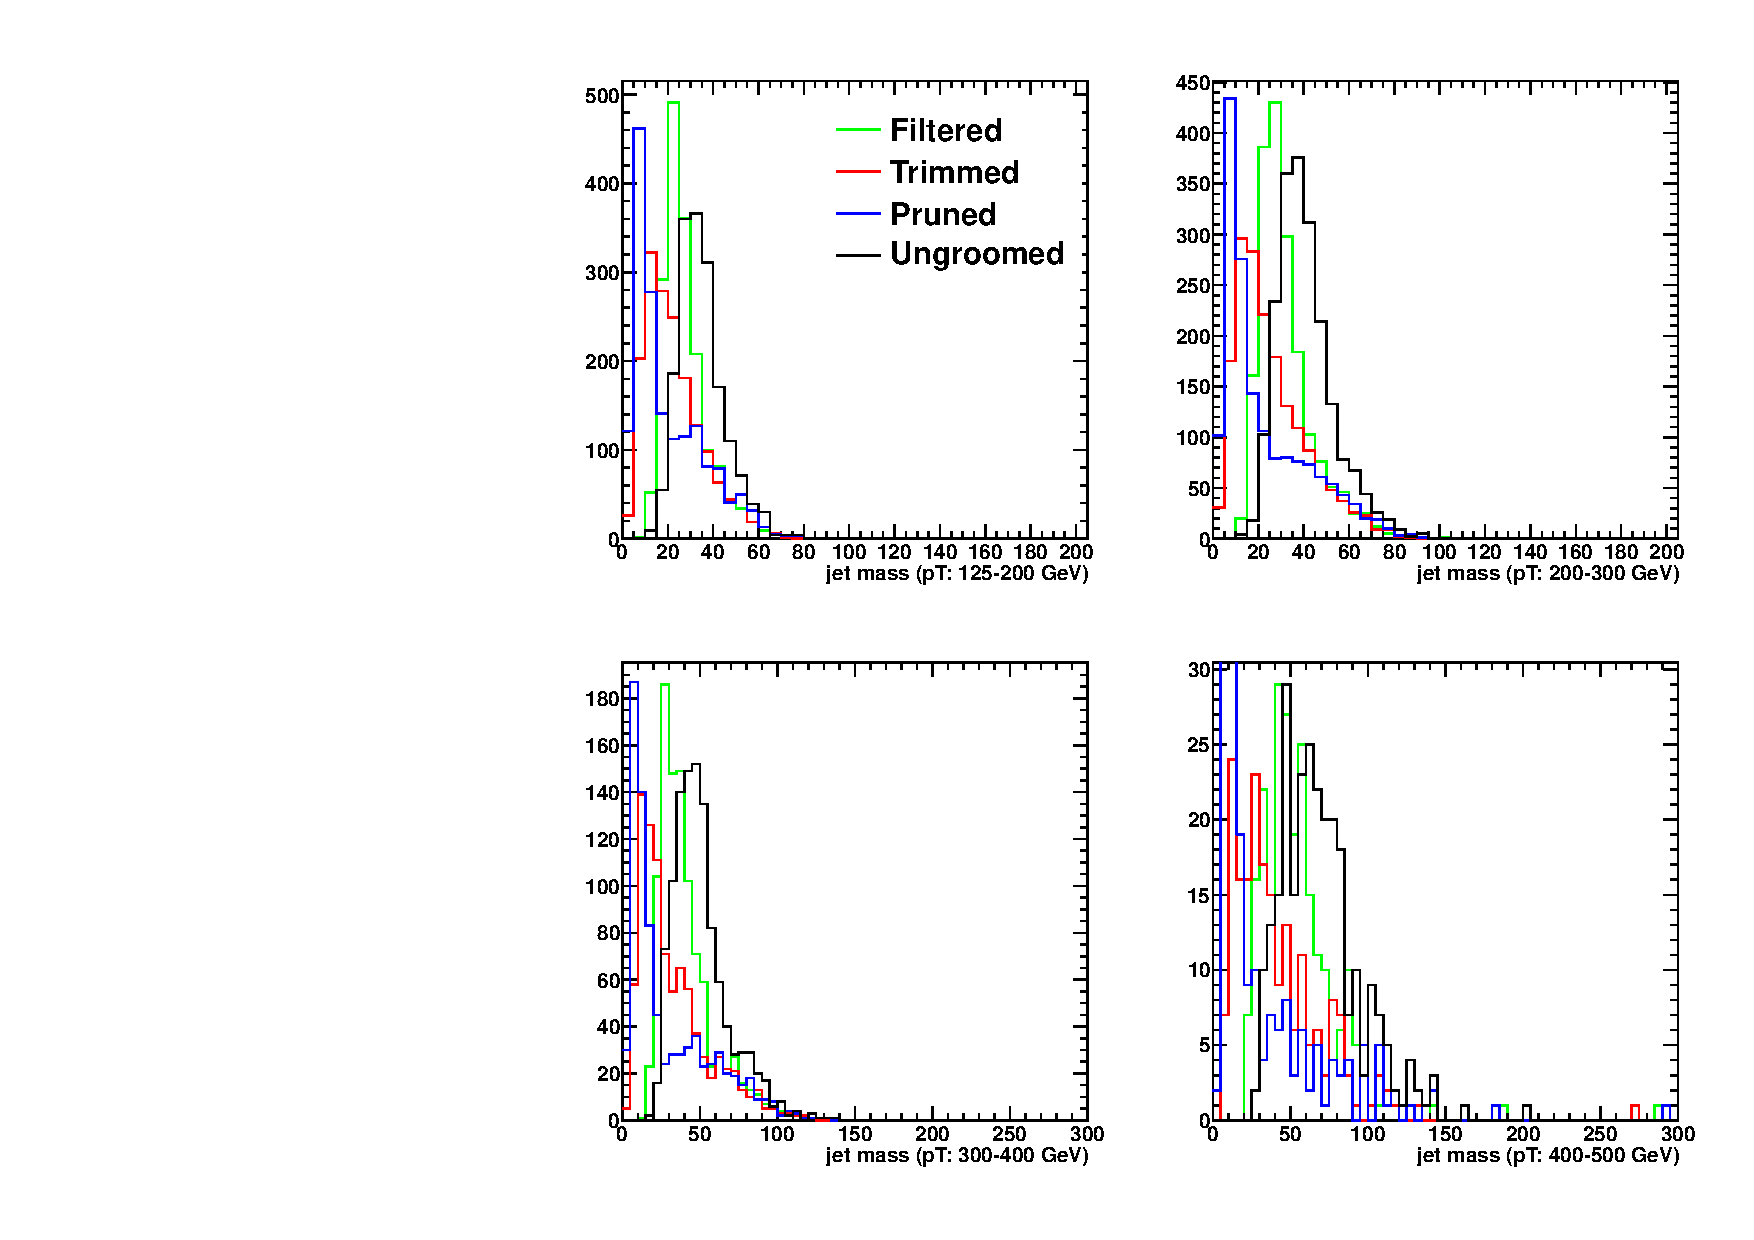
\includegraphics[width=1.0\textwidth]{figs/allAlgos_2x2PtBins_ak8.pdf}
\caption{Raw jet mass distribution on data for the leading AK8 (ungroomed or groomed) jet in different jet momentum regions.}
\label{figs:allAlgos3}
\end{figure}



